\section{模型的建立与求解}

\begin{mgAlgorithm}
    \item 打开冰箱
    \item 把大象放进去
    \item 关上冰箱
\end{mgAlgorithm}

\subsection{相似性度量模型}

\subsubsection{度量角度的确立}

在对小学数学应用题的相似性度量过程中,通常会使用两个依据:

\begin{enumerate}
    \item 根据题干文字进行相似性比对,确定两道题目间题面的相似程度。
    \item 通过人工或机器学习的方式为题目根据知识点进行“标签化”,两道题目之间的标签重合越多,则越相似。
\end{enumerate}

实际上,进行“标签化”对题目进行相似性度量是较为科学且准确的,符合师生快速锁定同类题型进行巩固训练的实际需求,而光凭文本信息进行相似性度量的结果并不符合实际的教育需求。

但仅根据少量题目样本无法将“标签化”过程有效自动化,难以避免通过人工手段为题目加上知识点标签。考虑到平台运营的切实情况,人工进行“标签化”操作成本过大,且判断过程中人为主观因素较多,可能也会导致度量结果出现较大偏差。

因而,本文经过综合考虑,还是选择通过题干文字进行相似性比对进行相似性度量。

\subsubsection{度量过程的关键步骤}


本文将度量过程总结成四个关键步骤以便于读者理解,下文也将围绕这四个关键步骤进行展开:

\begin{enumerate}
    \item 文本预处理
    
    文本预处理是自然语言处理中的重要步骤之一,其目的是将原始的文本数据转换成计算机可以处理的形式。为了提高文本处理任务的效率和准确性,文本预处理是在进行后续分析处理的必要前置步骤。

    \item 借助LDA模型建立相似性矩阵
    \item 使用余弦相似度计算相似性结果
\end{enumerate}

\subsubsection{文本预处理}

首先需要对题目文本进行分词处理,以好通过词袋模型的方式将题目文本进行向量化,进行进一步的研究。因本文研究的题目大多处于中文语言环境下,故笔者考虑采用NLPIR分词系统对题目进行分词处理。本文为了研究方便,使用的是被广泛使用的开源中文分词工具jieba。另外也可以使用NLPIR分词系统达到相同效果。NLPIR分词系统是由中国科学技术大学自然语言处理与社会人文计算实验室开发的一款中文自然语言处理工具。它是基于统计和规则两种方法相结合的分词系统,能够对中文文本进行精准的分词和词性标注,完美契合本文的研究需要。

在分词处理的过程中,还需要分离并忽略标点符号、数字、停用词等词语的影响。详细的处理操作可以参考周萍老师在《语义分析及相似性度量方法》\cite{}研究中总结的预处理流程。但本文简化了处理流程,仅对分词结果进行了简单的标点符号排除与数字排除,以加快研究进程。

\begin{figure}[htbp]
    \centering
    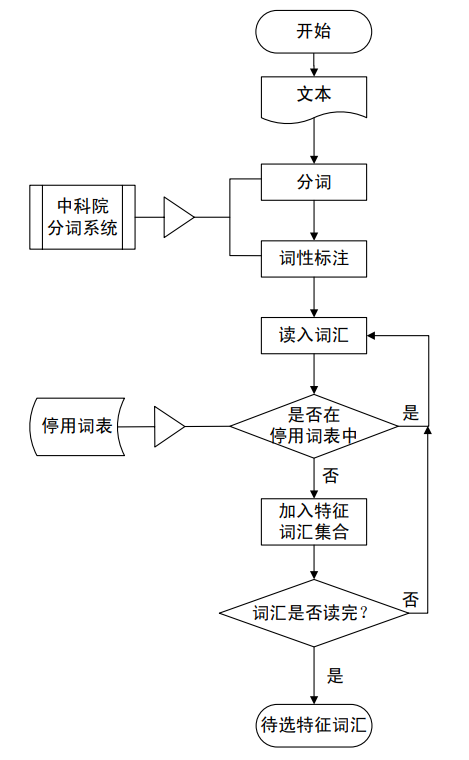
\includegraphics[width=6cm,height=10cm]{res/Text preprocessing process.png}
    \caption{文本预处理流程图}
\end{figure} 

在这里也给出一段进行文字预处理的Python代码以作参考,并作为后续研究的前提:

\begin{mgCodeBlock}[Python 文字预处理代码]
    \VerbatimInput{res/participle.py}
\end{mgCodeBlock}

\subsubsection{文本预处理}


\begin{mgCodeBlock}[C++ Hello World!]
\begin{verbatim}
    代码内容
\end{verbatim}
\end{mgCodeBlock}

\subsection{基于模糊数学的难度度量模型}

相对于研究和处理确定性现象的数学理论和方法,模糊数学是研究和处理模糊性现象的一种数学理论和方法\cite{}。对于一个题目来说,其难度与很多因素有关,并且很难量化地用这些因素来表示一个题目的难度,即一个题目的难度只能用模糊的标准来表示。而模糊数学在题目难度估计方面可以起到很好的作用。因此,使用模糊数学的方法来对一个题目难度进行度量。

\subsubsection{确定难度度量指标}

对于一个题目来说,有很多因素能够影响其难度。首先,影响一个题目难度最深的因素,是该题目所用到的\textbf{知识点数量}。显然,当知识点数量越多,对学生解题要求越高,即题目越难。其次是该题目\textbf{数学运算的难度}。在满足学生发挥稳定、有充足时间、不受外界干扰等理想情况下,该题目数学运算越复杂,学生写对该题目的难度就越大,从而让该题目越难。再其次是\textbf{题目背景的复杂性}。如果题目直接把条件和问题表达清楚,那么这个题目就非常明确;然而很多时候题目中会出现含有故事背景、篇幅较长等各种其他情况,使题目条件不清晰,并且需要学生从中挖掘题目条件和问题。这类题目显然相对于上一种来说,难度更大。最后是教师的\textbf{个人主观难度判断}。

对于其他的因素,如学生的知识点掌握情况,本模型不考虑。

假定\textbf{题目难度度量因素集}$S_{factor}$,且有:
$$S_{factor} = \{ s_1, s_2, s_3, s_4 \}$$
其中$s_1$、$s_2$、$s_3$和$s_4$为四个影响题目难度的因素,分别代表知识点数量、数学运算的难度、题目背景的复杂性和个人主观难度判断。

\subsubsection{确定难度度量等级}

假定\textbf{题目难度得分矩阵}$M_{diff}$,其中$M_{diff}(i, j)$表示第$i$题第$j$个因素的得分等级。等级越高,该因素对该题目的难度,相较于其他题目同样的因素与对应的题目的难度来说,贡献越大,即题目越难。经过考虑,将其划分为五个等级,并且对于所有的$i \geq 1, 1 \leq j \leq 4$,有$M_{diff}(i, j)\in \{1, 2, 3, 4, 5\}$。

得到每个教师的题目难度得分矩阵后,分别对每一题每个因素求教师数量的平均值,设为最终的题目难度得分矩阵,即:
$$
M_{diff}(i, j) = 
    \frac{
        \sum_{k = 1}^{n}M_{diff}'(i, j, k)
    }{n}
$$

\subsubsection{确定难度度量权重}

假定\textbf{题目难度因素权重序列}$L_{weight}$,其中$L_{weight}(j)$表示第$j$个元素影响题目难度的权重,并且$1 \leq j \leq 4$。经分析,考虑:
$$L_{weight} = [4, 3, 2, 1]$$

由于题目难度得分矩阵不确定,并且对于不专业的人来说很难得到准确结果,考虑让多个教师合作完成。假定有$n$个教师分别完成各自的题目难度得分矩阵,\textbf{所有教师的题目难度矩阵}为一个三维矩阵$M_{diff}'$,其中$M_{diff}'(i, j, k)$表示第$k$个教师认为第$i$题第$j$个因素的得分,且有$i \geq 1, 1 \leq j \leq 4, 1 \leq k \leq n, M_{diff}'(i, j, k)\in \{1, 2, 3, 4, 5\}$。

\subsubsection{模糊综合评价}

构建题目难度度量模型之后,可以由此得到\textbf{难度值}$L_{diff}$,其中$L_{diff}(i)$表示第$i$题的难度值,并且满足$i \geq 1$。由建立的模型可得对应题目难度的加权值为:
$$
L_{diff}(i) = 
    \sum_{j = 1}^{4} \left [ 
        M_{diff}(i, j) \cdot L_{weight}(j)
    \right ]
$$

由于本题目难度度量模型针对的是附件中题库内的所有题目,对于每一题来说,难度值都是相对于题库内所有题目的难度值而言。假定题目相较于题库中其他题目的难度为\textbf{难度系数}。所有题目的难度系数序列为$L_D$,其中$L_D(i)$表示第$i$题的难度系数,且有$i \geq 1$。则难度系数的计算方式为:
$$
L_D(i) = 
    \frac{
        L_{diff}(i)
    } {
        \max L_{diff}
    }
$$
其中$\max L_{diff}$为题库中题目最大的难度值,并且有$0 < L_D(i) \leq 1, i \geq 1$。

至此,题库中所有题目的难度均度量完成,即$L_D$。

\subsection{}

% ============================================================
%
% 模型的评价与改进
%
% ============================================================

\section{模型的评价与改进}

\subsection{模型的优点}

\begin{itemize}
    \item 12
\end{itemize}

\subsection{模型的缺点}

\subsection{模型的改进}